\documentclass[../thesis.tex]{subfiles}

\begin{document}

\chapter{Introduction}\label{chp:Introduction}

This research project has been conducted in collaboration with Clinical Futures within the Aneurin Bevan University Health Board (ABUHB) \cite{UniAneurinBevanHealthBoard} and is funded jointly by the Welsh Government's European Social Fund (ESF) convergence programme for East Wales and the Knowledge Economy Skills Scholarship (KESS2) \cite{KESS2023}. Clinical Futures is the Health Board's plan for sustainable health and care services for the NHS across South East Wales. The organisational structure of bed capacity and personnel resource planning within ABUHB is examined in this thesis, specifically for the elderly and frail patient demography.

In the United Kingdom (UK), the National Health Service (NHS) is a publicly funded healthcare system \cite{Welch2018}. Founded in 1948, the principle was that services should be comprehensive, universal and free at the point delivery, with the basis for health care being clinical need rather than financial capability. It is the second largest single-payer healthcare system in the world and in 2021 accounted for $\pounds$229 billion of the UK Government's annual spending \cite{ONS2022a}.


\section{Elderly and Frail Patient Demographics}\label{sec:elderlyfrail}
Due to declining fertility and mortality rates as well as increased life expectancy, many countries are dealing with an ageing population. Additionally, those who were born during the post world war two baby boom, are now aged 60 or older. These factors are among the key causes behind the United Nations 
(UN) prediction that by 2050, one in six people worldwide, and one in four in Europe, will be aged over 65. According to the UN \cite{UN3}, in 2018 there were more people aged 65 and older than children aged under five worldwide for the first time in history. In healthcare research, elderly patients are commonly defined as individuals who are aged 65 and older \cite{Crews2006,GOV.UK2001,NHSEngland,Orimo2006}. This definition will be applied throughout this thesis. 


Within the UK in 2022, 18.65\% of residents are aged 65 and over (approximately, 12.5 million), of which 8.63\% are aged 75 and over \cite{ONS2022b}. The population's share of those aged 90 and older is thought to be around 0.91\%. With 21.09\% of the population over the age of 65, Wales has a proportionally larger elderly population than the rest of the UK. Those aged 75 and older account for 9.68\% with 0.97\% of the population being aged 90 and over. Figure \ref{fig:PopulationPyramids} displays the population pyramids for the Welsh population from the 2001 and 2021 censuses, together with the estimated population for 2031. The 2011 pyramid demonstrates stationary growth, which is defined as the population remaining constant in different age groups. The 2021 and 2031 pyramids depict the start of a constrictive pyramid, in which the number of new births are low, and the population is ageing. Between 2020 and 2030, the Welsh Government projects a 16.1\% growth in the population aged 65 and over. This rises to an increase of 23.9\% for those aged 75 and over between 2020 and 2030 \cite{WelshGovernment2022}.




\begin{figure}[h!]
\centering
\begin{subfigure}{0.33\textwidth}
    \centering
    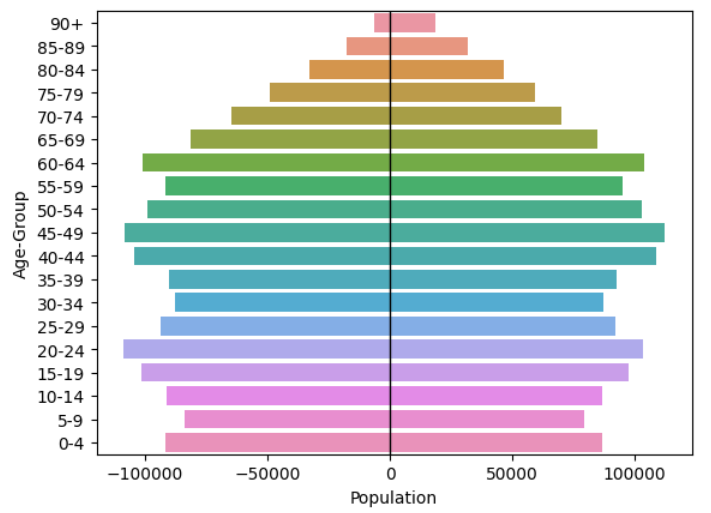
\includegraphics[width=\textwidth]{Chapters/Chapter1/Figures/Census2011.png}
    \caption{2011}
\end{subfigure}
\hfill
\begin{subfigure}{0.33\textwidth}
    \centering
    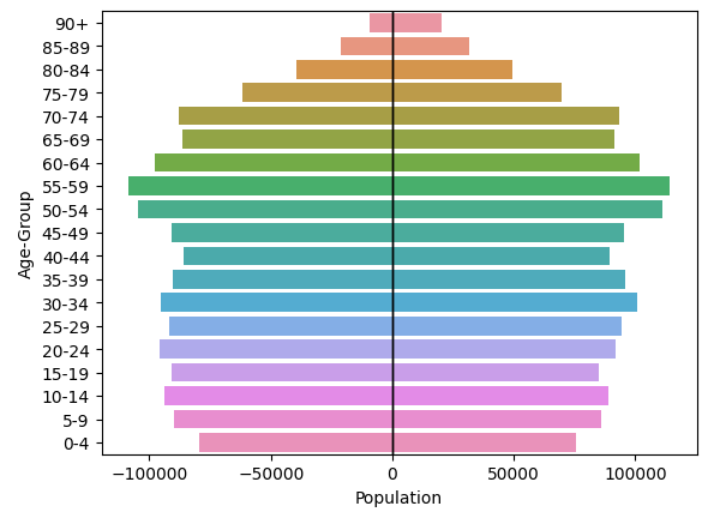
\includegraphics[width=\textwidth]{Chapters/Chapter1/Figures/Census2021.png}
    \caption{2021}
\end{subfigure}\hfill
\begin{subfigure}{0.33\textwidth}
    \centering
    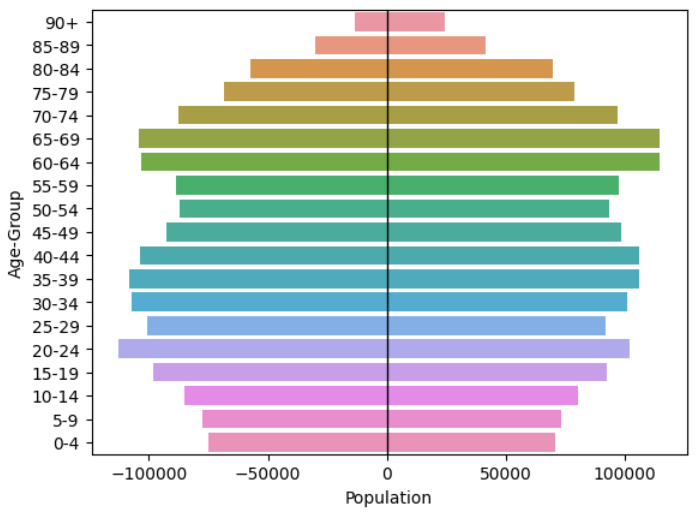
\includegraphics[width=\textwidth]{Chapters/Chapter1/Figures/Census2031.png}
    \caption{2031}
\end{subfigure}
    \caption{Population Pyramids for the Years: 2011, 2021 and 2031}
    \label{fig:PopulationPyramids}
\end{figure}


%Cite these:
%https://assets.publishing.service.gov.uk/government/uploads/system/uploads/attachment_data/file/198033/National_Service_Framework_for_Older_People.pdf
%https://www.england.nhs.uk/ourwork/clinical-policy/older-people/improving-care-for-older-people/
%https://www.researchgate.net/publication/263589932_Reviewing_the_definition_of_elderly
%https://www.jstage.jst.go.jp/article/jpa2/25/1/25_1_113/_article/-char/ja/

%https://assets.publishing.service.gov.uk/government/uploads/system/uploads/attachment_data/file/198033/National_Service_Framework_for_Older_People.pdf


Frailty is described as having a high risk of falling into dependency as a result of a negative event, such as an accident, fall or disability. Despite the fact that frailty is more common as people get older, it develops independently from ageing \cite{Topinkova2008}. Since there is no international standard of measurement for frailty, this is challenging to categorise and monitor \cite{Dent2016}. This means that determining whether or not a person is frail frequently depends on clinical judgement. Even in the UK, there are various ways to determine frailty, such as the clinical frailty score \cite{Rockwood2005} and the electronic frailty score \cite{NHSEnglanda}. According to estimates from Age UK \cite{AgeUK2020}, 10\% of over 65's live with frailty, and the percentage rises to between 25\% and 50\% for those over 85.

Within this research, a frailty score was created using a combination of two methods (\cite{Gilbert2018, Soong2015}), on the hospital disease codes, also known as the International Statistical Classification of Diseases and Related Health Problems - 10$^{th}$ revision (ICD10) \cite{NHSWales}. The ICD10 code, which was first mandated for use in the UK in 1995, provides descriptions of all recognised diseases and injuries. Each condition is detailed with diagnostic characteristics and given a unique identifier that is used to code morbidity data from patient and clinician records as well as mortality data on death certificates. The ICD10 has a minimum of three characters, and a maximum of four characters can be added to provide more information about the diagnosis. An example of the breakdown of an example ICD10 code is shown in Table \ref{tab:icd10}:

\begin{table}[h!]
    \centering\scalebox{0.9}{
    \begin{tabular}{p{8cm}cccccccc}\toprule
         &  \multicolumn{3}{c}{Category} & &  \multicolumn{3}{c}{Subcategory} & Extension\\\midrule
        Description & 1$^{st}$& 2$^{nd}$& 3$^{rd}$& & 4$^{th}$& 5$^{th}$& 6$^{th}$ & 7$^{th}$\\\midrule
        Fracture of shoulder and upper arm & S & 4 & 2 \\
        Fracture of upper end of humerus & S & 4 & 2 & . &2 \\
        Unspecified fracture of upper end of humerus  & S & 4 & 2 & . &2 &0\\
        Unspecified fracture of upper end of right humerus& S & 4 &2&.&2&0&1\\
       {Unspecified fracture of upper end of right humerus - initial encounter for closed fracture} & S & 4 &2&.&2&0&1 & A\\\bottomrule
    \end{tabular}}
    \caption{Breakdown of the Example ICD10 Code - S42.201A}
    \label{tab:icd10}
\end{table}

Gilbert et al. \cite{Gilbert2018} developed a hospital frailty risk score, where certain ICD10 codes were more than twice as likely to be present in a frail patient compared to a non-frail patient. This scoring system has a range of 0.1 to 7.,1 where a higher score suggests a higher proportion of frail patients within the groupings. Soong et al. \cite{Soong2015} generated a list of syndromes which were more common within frailty patients, where if a syndrome is present then a score of one is given. To assure coverage of all frailty syndromes, the two score measures were combined because they each contained different ICD10 codes. This yields a range from 0 (where there is no frailty syndrome present) to 8.1, the highest scoring frailty syndrome.

%https://www.ageuk.org.uk/our-impact/policy-research/frailty-in-older-people/understanding-frailty/#:~:text=Frailty%20is%20generally%20characterised%20by,for%20those%20aged%20over%2085.
%\hl{I need to talk about how we are measuring frailty - the two scoring techniques}
% page 7 graph do something similar for wales
% definition
% \begin{itemize}
%     \item aging population
%     \item more movement of people in wales %https://www.ons.gov.uk/peoplepopulationandcommunity/populationandmigration/populationestimates/bulletins/populationandhouseholdestimateswales/census2021
%     \item percentage make up of over 65
%     \item Levels of deprivation - in abuhb section
% \end{itemize}


\section{Aneurin Bevan University Health Board}\label{sec:ABUHB}

The Aneurin Bevan University Health Board (ABUHB) was established in 2009 and serves 650,000 residents located in five counties: Blaenau Gwent, Caerphilly, Monmouthshire, Newport and Torfaen, as well as some areas of South Powys (Figure \ref{fig:AbuhbCounties}). Two-thirds of the health board's 14,000 personnel work directly with patients \cite{UniAneurinBevanHealthBoardb}. The health board has direct links with applying operational research (OR) and modelling to improve healthcare decisions with a team of analysts embedded within the organisation forming the Aneurin Bevan Continuous Improvement team (ABCi) \cite{UniAneurinBevanHealthBoarda}.

\begin{figure}[h!]
    \centering
    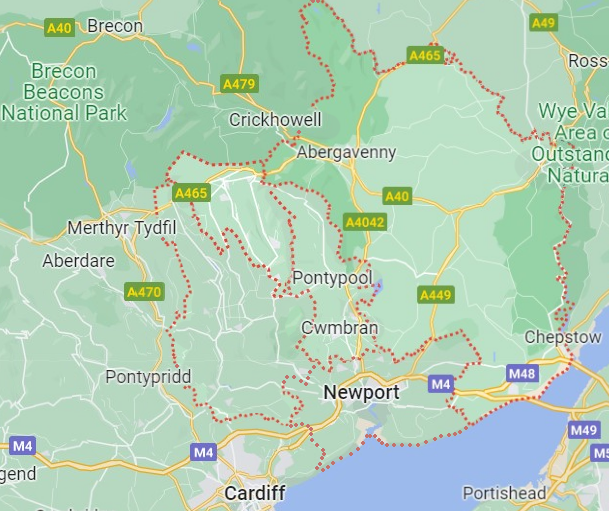
\includegraphics[scale=0.8]{Chapters/Chapter1/Figures/ABUHBmap1.png}
    \caption{Aneurin Bevan University Health Board}
    \label{fig:AbuhbCounties}
\end{figure}

Clinical Futures is the Health Board's plan for sustainable health and care services for the NHS across the Gwent area. General practitioners (GP) practices, emergency rooms, and longer wait times for services that a large number of people require, such orthopaedic and ophthalmology care, are dramatically putting greater strain on the whole healthcare system. Their aim is to deliver effective and efficient care in hospitals while planning across all services to keep people out of hospital. Clinical Futures is reforming the organisation to provide more centralised hospital treatment for individuals in need, as well as care closer to home, in order to satisfy these demands and succeed in `The Wellbeing of Future Generations Act (2015)' \cite{WelshGovernment} (Figure \ref{fig:ClinicalFutures}).

\begin{figure}[h!]
    \centering
    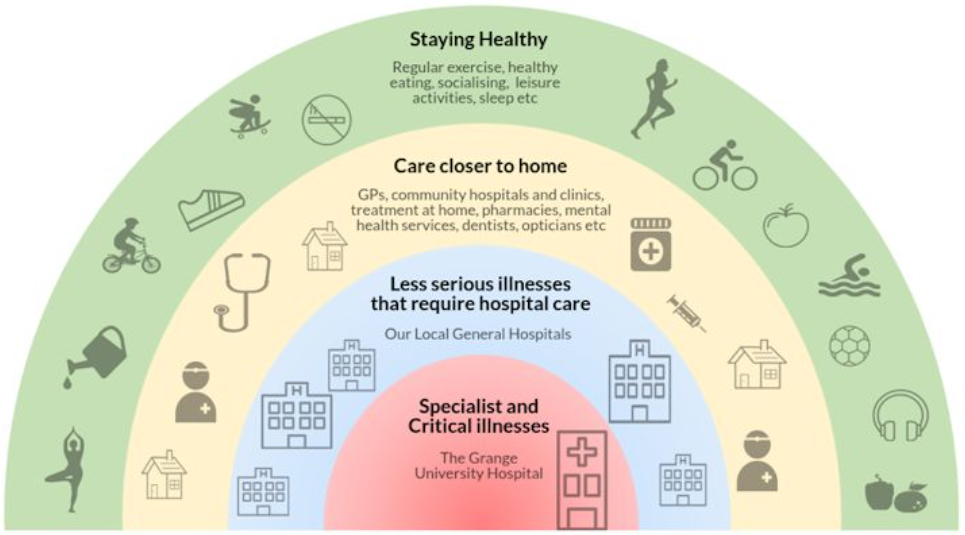
\includegraphics[scale=0.8]{Chapters/Chapter1/Figures/Clinical Futures.png}
    \caption{Clinical Futures Future Healthcare Plan \cite{UniAneurinBevanHealthBoard2018}}
    \label{fig:ClinicalFutures}
\end{figure}

The health board comprises of eleven hospitals providing different levels of care. A specialised critical care centre called The Grange University Hospital (GUH) opened earlier than expected in November 2020 to offer more assistance during the Covid-19 pandemic. Inpatient stays at GUH will not have been included because the primary emphasis of this study is on data collected before the Covid-19 epidemic. The model developed within this thesis will have the ability to be adapted to changing services throughout the health board in the future, including the addition of GUH.
There are four minor injury units (MIU's), one acute hospital and five community hospitals (Table \ref{tab:hospitals}).

\begin{table}[h!]
    \centering\scalebox{0.8}{
    \begin{tabular}{ll} \toprule
      \textbf{Hospital Type}   & \textbf{Hospital Name} \\\midrule
       Major A\&E Unit  & The Grange University Hospital (GUH) \\
       Minor Injury Unit (MIU) & Nevill Hall Hospital (NHH), Royal Gwent Hospital (RGH), \\
       &Ysbyty Aneurin Bevan (YAB), Ysbyty Ystrad Fawr (YYF)\\
       Acute Hospitals & St. Woolos Acute Hospital (STWAH)\\
       Community Hospitals & Chepstow Community Hospital (CCH), County Hospital (CH),\\ &Monnow Vale Health \& Social Care Facility (MVHSCF), St. Woolos \\ &Community Hospital (STWCH), Rhymney Integrated Health \& Social Care Centre (RIHSC)\\\bottomrule
    \end{tabular}}
    \caption{Type and Names of Hospitals Located in ABUHB}
    \label{tab:hospitals}
\end{table}

These hospitals are spread throughout the health board, with one major accident and emergency (A\&E) unit or MIU in each county (Figure \ref{fig:abuhblocations1} shows major A\&E unit in red and MIU's in orange). Figure \ref{fig:abuhblocations1} depicts the community hospitals, which are dispersed around the health board and are shown in purple.

\begin{figure}[h!]
    \centering
    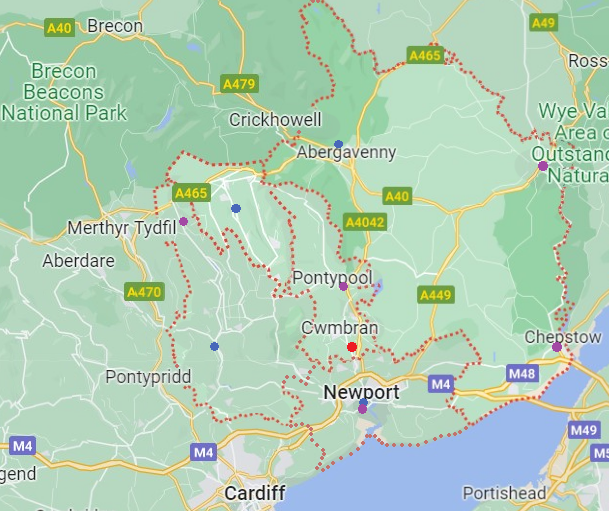
\includegraphics[scale=0.9
]{Chapters/Chapter1/Figures/ABUHBmap3.png}
    \caption{Map of Hospital Locations in ABUHB - Major A\&E Unit Shown in Red, MIU's Shown in Blue, Acute and Community Hospitals Shown in Purple.}
    \label{fig:abuhblocations1}
\end{figure}


Each hospital offers patients different inpatient services. There are a total of 29 specialisations offered by the area. How specialties are currently organised in each of these hospitals is shown in Figure \ref{fig:hospspec} (as of March 2020). There are 98 unique hospital and specialty pairings in total. More specialties are found in larger, more acute hospitals, such as RGH, which has 25, as opposed to fewer specialties in smaller hospitals like County Hospital (CH). Appendix \ref{App:Hospitals} has a complete list of hospitals, along with a summary of the specialties that each one offers.

\begin{figure}[h!]
    \centering
    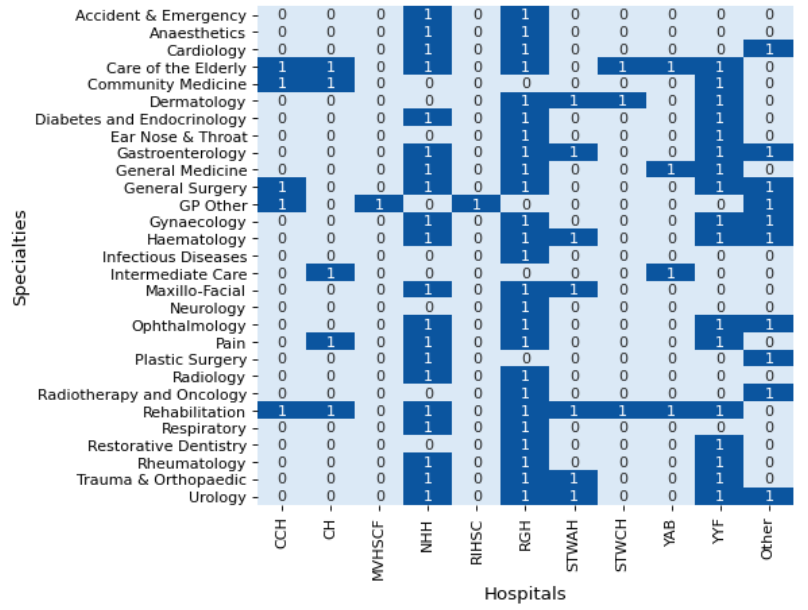
\includegraphics[scale=0.9]{Chapters/Chapter1/Figures/Hospitalloc19.png}
    \caption{Hospitals and Specialties in the ABUHB, with 1 Indicating a Specialty is Present in a Given Hospital and `0' Indicating a Specialty is Not Present}
    \label{fig:hospspec}
\end{figure}


%Within ABUHB there are ten main hospitals, divided into four acute and six community hospitals (Figure \ref{fig:Hospital}). Additionally, there were four more locations included within the data: `Offsite', `Outsource', `Outsource - Care UK' and `University Hospital Wales'. The first three locations are run by private or specialist care providers. University Hospital Wales is located in the Cardiff and Vale health board region, however was included within analysis since patients are often transferred to this hospital when demand cannot be met.

% \begin{itemize}
%     %\item Talk about Grange opening
%     %\item At some point in this chapter mention KESS
%     %\item Talk about types of services that are offered within the health board
%     %\item deprivation in the region
%     %\item individuals over X by local area
%    % \item https://towardsdatascience.com/mapping-with-matplotlib-pandas-geopandas-and-basemap-in-python-d11b57ab5dac
%    % \item issues in bed planning
%    % \item overcrowding etc. bed blocking
%    % \item maybe separate section of issues in healthcare with frail and elderly patients?
%    % \item talk about how much additional hospital time elderly and frail patients stay in hospital - how much additional staffing resources
% \end{itemize}

% \begin{figure}[H]
%     \centering
%     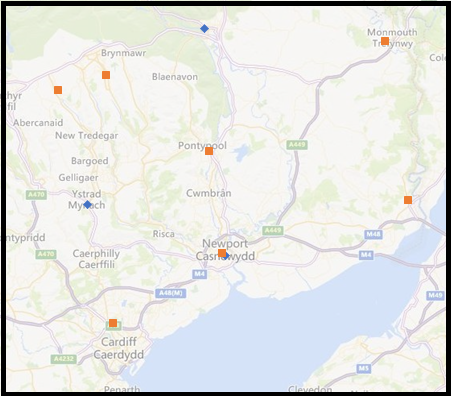
\includegraphics[width = 8cm]{Chapters/Chapter1/SE Wales.png}
%     \caption{Map of Acute Hospitals (Blue) and Community Hospitals (Orange) in South East Wales. \hl{Can look at improving map}}
%     \label{fig:Hospital}
% \end{figure}

% \begin{itemize}
%     \item step up and step down care
%     \item differences between acute community
% \end{itemize}
\section{Bed Planning and Staff Allocation}
Figure \ref{fig:bedmanagement} shows a patient's journey after being admitted to an acute ward. Patients may be admitted as elective or emergency patients. Patients who are unexpectedly and quickly admitted to the hospital are considered emergency admissions. These patients may be accepted through GPs or consultants in ambulatory clinics, as well as A\&E units. According to Steventon et al. \cite{Steventon2018}, the number of emergency admissions is rising at an average of 3.2\% year. Elective patients receive scheduled care, frequently involving expert clinical treatment or surgery, and are typically referred by a GP or other community health provider.

Patients who are admitted to the hospital, whether on an elective or emergency basis, remain there until they are deemed to be `medically fit to be discharged'. Patients discharges can frequently be delayed for a variety of reasons, such as waiting for home care, waiting for a permanent bed in a nursing or care facility  or awaiting a medical decision and full discharge summary. The home first approach \cite{NHSEnglandb}, strives to discharge patients with long-term care needs to an appropriate setting, where assessments of what care they require and how it will be financed take place (Care and nursing homes in the UK are typically funded by the patient). This approach is crucial for maximising health outcomes. Most patients leave hospital and go home without any more assistance. However, the majority of patients who encounter delays to discharge require community care and typically, these patients are older adults.

\begin{figure}[h!]
    \centering
    
\includegraphics[scale=0.6]{Chapters/Chapter1/Figures/bedmanagement.png}
    \caption{Conceptual overview of the patient journey and the role of bed management.} %https://emj.bmj.com/content/20/2/149}
    \label{fig:bedmanagement}
\end{figure}



Figure \ref{fig:Piechartdelays} shows that the main reason patients experience delays to discharge are a lack of access to the services that are best for them, with home care accounting for 24\% of delays, short-term rehabilitation accounting for 22\% of delays, and care/nursing homes accounting for 15\% of delays. These figures indicate that the capacity of community services is severely constrained. As a result, new patients cannot be admitted since the beds are occupied by people who are waiting to be discharged and this is known as bed blocking.

\begin{figure}[h!]
    \centering
    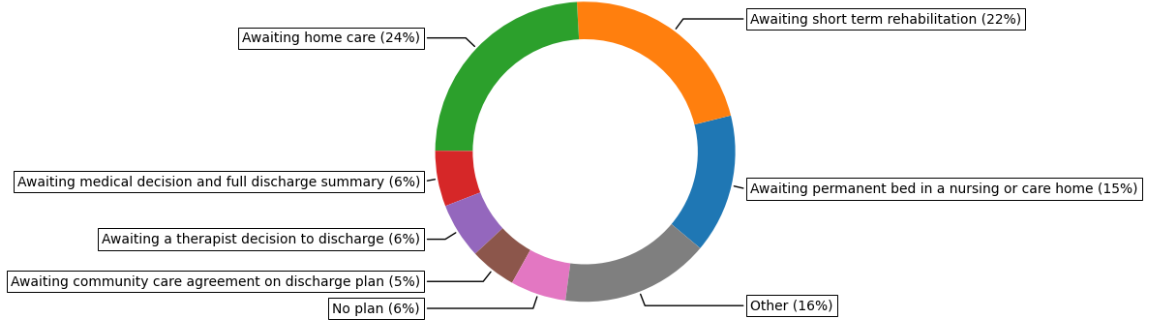
\includegraphics[scale=0.7]{Chapters/Chapter1/Figures/piechart.png}
    \caption{Reason for Delayed Discharge for Patients with aLength of Stay (LOS) Longer than a Week \cite{NuffieldTrust2022}}
    \label{fig:Piechartdelays}
\end{figure}

Elective patient operations are cancelled to make way for priority emergency admissions when the capacity is insufficient and the beds are full. Similarly, planned admissions are frequently cancelled and wards are altered in order to securely meet ward criteria if there are insufficient nursing staff. The Nurse Staffing Levels (Wales) Act 2016 \cite{NHSAct2006}, was the first law passed in the UK requiring that health boards provide sufficient nursing staff so all patients receive compassionate care. This requires a designated individual to determine the number of nurses necessary to provide care to patients that satisfies all reasonable requirements in each situation. Additionally, they must take all responsible steps to maintain the nurse staff level. This relies on one individual to utilise expert judgement and can be problematic when deciding on the final personnel levels. Staff planning must take into account uplift, and capacity should accommodate anticipated and planned changes in the number of nursing staff members available (e.g., annual leave, training, study leave).

Equation \ref{eq:staffplanning} displays the method of allocating ward nursing staff in order to calculate the typical nursing staff demand for a 24 hour period \cite{NIHCE2014}. 

\begin{align}\label{eq:staffplanning}
    \text{Average Requirement} =& \text{Average Hours Per Patient} * \text{Average Daily Bed Utilisation } + \notag \\ &\text{Additional Workload in Nursing Hours Per Day}
\end{align}


%\subsection{Bed Planning}
The main challenges faced by healthcare managers are the hundreds of beds and staff to manage, which creates an excessive number of options for decisions. Demand and capacity are further complicated because no two patients are exactly alike. Because bed capacity planning typically relies on averages, it fails to take into consideration the stochastic nature of the healthcare industry \cite{Harper2002}. By utilising OR approaches, this thesis seeks to enhance planning for both beds and staff.



\section{Research Aims}\label{sec:researchaims}
To address the organisational needs within the NHS, four research questions were established in partnership with senior staff from Clinical Futures and ABUHB.

\begin{enumerate}
   % \item How will admissions for the elderly and frail patient community within ABUHB change over time? #How do certain factors
    \item How do the clinical and demographical attributes of elderly and frail patients effect their length of stay within hospital? 
    
    %\item What is an efficient way to organise specialties among a network of hospitals to ensure staffing and bed costs are minimised? OR\\
    \item How best can specialities be organised among a network of hospitals to ensure staffing and bed costs are minimised? %organised change word
    
    \item How can deterministic and two-stage stochastic models be used to successfully plan hospital services?%Be more specific - what model
    \item How can linking predictive and prescriptive analytics increase the reliability of the models?
\end{enumerate}

\section{Thesis Structure}
This thesis consists of eight chapters, together seeking to answer the four research questions described in Section \ref{sec:researchaims}. The structure of the thesis is as follows:

\begin{itemize}
\item Chapter \ref{chp:Introduction} has contextualised four main research questions of this thesis. Background into the ABUHB has been discussed, with the major problems in planning of beds and staffing for elderly and frail patients.
    \item Chapter \ref{chp:LiteratureReview} contains two literature reviews: The first comprising of \cite{Williams} discusses the application of OR techniques within elderly and frail patient care and the second discusses hierarchical prediction models for patients' length of stay (LOS). These literature reviews provide an insight into the type of OR models that are currently used in this field of study and the opportunities available for researchers to conduct future study.
    
    \item Chapter \ref{chp:predictive} discussed the theory on the predictive modelling techniques that have been will be applied to health board data in Chapter \ref{chp:Experimental Analysis}. The concept of classification and regression trees are introduced with explanation in how these methods can be implemented with Python. Discussion into the application of bed and staff planning is also given.
    
    \item Chapter \ref{chp:presciptive} discussed the theory of prescriptive modelling. Deterministic and two stage stochastic models are developed which aims to minimise overall costs by optimally planning bed and nursing resources. This theory will be applied to a case study of elderly and frail in ABUHB within Chapter \ref{chp:Experimental Analysis}.

    
    \item Chapter 5 \hl{To be written - once chapter completed}    
    \item Chapter \ref{chp:Linking} \hl{To be written - once chapter completed}
    \item Chapter 7 \hl{To be written - once chapter completed}
    \item Chapter 8 \hl{To be written - once chapter completed}
    
\end{itemize}
\end{document}
